\chapter{FUNDAMENTAÇÃO TEÓRICA}\label{fund}

É objetivo deste capítulo descrever o referencial teórico tido como base para a elaboração do presente trabalho. Para tanto, foi desenvolvido um modelo incremental quanto a solução de desafios encontrados no decorrer do seu desenvolvimento.

Inicialmente são apresentadas as DTNs por meio de uma contextualização e definição dos principais conceitos relacionados. A partir daí, as principais aplicações existentes são explanadas e seus principais desafios apresentados. A partir daí é proposto um modelo de gerenciamento inteligente da energia das baterias baseado em Gradientes de Concentração e Geolocalização.

Após a apresentação das DTNs, o conceito de Gradientes de Contração são explorados por meio de uma contextualização intuitiva, sua definição e, finalmente, a proposta de aplicação dos mesmos nas DTNs, apresentando, para isto, uma solução baseada em Geolocalização para o mapeamento geográfico.

Em seguida, os Sistemas de Navegação por Satélites são explanados. A abordagem segue a mesma linha dos tópicos anteriores, ou seja, parte-se da contextualização e definição para a aplicação dentro do âmbito das DTNs.

Por fim, é realizada a conclusão, onde ocorre o fechamento deste capítulo.

\section{Redes Tolerantes a Atrasos e Desconexões}\label{sec:DTN}

Nesta seção é realizada uma breve análise sobre a arquitetura atual da Internet, seus protocolos e suas respectivas dificuldades para trabalhar em cenários para os quais não foram projetados. Além disso, é apresentada a fundamentação teórica necessária sobre as Redes Tolerantes a Atrasos e Desconexões, incluindo definição, arquitetura e os principais desafios existentes.

\subsection{Contexto}\label{sec:DTN_contexto}

A Internet é uma grande rede de computadores de imenso sucesso. A importância da sua organização é de fácil percepção, visto a grande quantidade de possibilidades oferecidas e o seu desempenho satisfatório. 

A arquitetura da Internet é baseada em um modelo referência denominado modelo OSI (do inglês "\emph{Open Systems Interconnection}" ou "Interconexão de Sistemas Abertos", em português), que estabelece uma arquitetura em camadas, sendo, cada uma delas, responsável por implementar serviços inerentes a uma determinada etapa da comunicação entre os dispositivos. 

Protocolos de comunicação são responsáveis por implementar os serviços de uma determinada camada. Tais protocolos são definidos por meio de RFCs (do inglês "\emph{Request For Comments}" ou "Pedido para Comentários", em português), documentos técnicos desenvolvidos e mantidos pela  IETF (do inglês "\emph{Internet Enginnering Task Force}" ou "Força Tarefa de Engenharia da Internet", em português), que, por sua vez, é uma instituição responsável por especificar os padrões a serem implementados na Internet.

Destacam-se, dentre todos os protocolos utilizados na Internet, o TCP (do inglês "\emph{Transmission Control Protocol}", ou "Protocolo de controle de transmissão") e o IP (do inglês "\emph{Internet Protocol}" ou "Protocolo da Internet"). Tais protocolos são a base da maioria das trocas de dados entre os hospedeiros\footnote{Hospedeiros são dispositivos que executam aplicações. Smartphones, laptops, computadores de mesa e PDAs são exemplos clássicos de hospedeiros\cite{kurose2010redes}.} da Internet. 

Sobre a Internet e seus dois principais protocolos, o TCP e o IP, valem as afirmações \cite{kurose2010redes}:

\begin{itemize}
    \item \textbf{Infraestrutura Dedicada:} Existem grandes corporações da área de telecomunicações e instituições sem fins lucrativos envolvidas na organização da arquitetura da Internet, seja realizando a sua manutenção ou criando novos protocolos, aumentando e melhorando a infraestrutura existente ou criando novos acordos internacionais visando a melhoria da transmissão de dados;
    \item \textbf{Existência de um caminho fim-a-fim:} Os protocolos da Internet seguem um modelo de comunicação que pressupõe a existência de ao menos um caminho fim-a-fim entre dois nós\footnote{Nós são os dispositivos que compõem uma rede, sendo os hospedeiros um exemplo deles.}. Tal caminho torna possível estabelecer uma conexão entre dois hospedeiros quaisquer conectados a Internet a qualquer momento. De fato, esse pressuposto é sempre atendido na Internet, principalmente pela imensa infraestrutura existente e os grandes investimentos realizados pelas corporações;
    \item \textbf{Confiabilidade:} O protocolo TCP tem como principal premissa a transferência confiável de dados entre os dispositivos. A confiabilidade é implementada utilizando técnicas de verificação de erros e retransmissão de mensagens quando algum erro é detectado;
    \item \textbf{Estabilidade:} Mesmo com a inexistência de garantias de atraso e largura de banda\footnote{Largura de banda é uma grandeza utilizada para medir o quão rápido se dá uma troca de dados entre dispositivos de computação. É mensurada como bits por segundo.}, a Internet é caracterizada por baixas taxas de atraso fim-a-fim e perdas de dados. Isso se deve ao fato de as empresas envolvidas sempre se preocuparem com a melhoria, manutenção e expansão da infraestrutura existente.
\end{itemize}

Existem cenários que as afirmações válidas na Internet não podem ser realizadas, como os ambientes definidos pela ausência de uma infraestrutura dedicada, problemas associados a mobilidade e limitações de hardware dos dispositivos. Esses ambientes comprometem seriamente o funcionamento dos protocolos TCP e IP, trazendo muitos desafios de conectividade entre os nós. Redes assim caracterizadas, como já introduzido, são conhecidas como DTNs (do inglês "Delay Tolerant Networks") ou \emph{Redes Tolerantes a Atrasos e Desconexões} \cite{alves2009redes}.

As DTNs são amplamente utilizadas para prover conexões em situações desafiadoras como as anteriormente apresentadas, possibilitando a troca de dados em lugares onde não é possível evitar altas taxas de latência e desconexões. Exemplos mais detalhados de aplicações são apresentados na subseção \ref{sec:aplicacoes}.

\subsection{Definições}\label{sec:definicoes}

As Redes Tolerantes a Atrasos e Desconexões são redes de computadores caracterizadas, principalmente, por conexões sem fio e ausência de infraestrutura dedicada para a troca de dados entre os dispositivos que a compõe, tornando necessário a cooperação dos nós para que ela seja autossuficiente. 

A mobilidade é uma importante característica das DTNs, tornando a topologia variante no tempo e, devido a falta de infraestrutura dedicada, existe a ausência de garantias de conexão intermitente entre os nós. As DTNs sofrem, ainda, com altas taxas de latência e desconexões \cite{fall2003delay}, sendo comum estarem na ordem de horas a, até mesmo, dias.

A utilização de dispositivos sem-fio limita a comunicação em um pequeno espaço geográfico, pois torna necessário que um nó esteja na área de alcance do outro para trocarem dados. Esse curto alcance dos dispositivos atrelado à mobilidade torna a cooperação um elemento básico nessas redes, pois, quando um remetente precisa contatar um outro nó que não está em sua área de alcance, este pode repassar a mensagem para um ou mais nós intermediários acessíveis, esperando que eles possam entregar a mensagem em um momento oportuno, seja para outros nós intermediários ou para o próprio destinatário. Confiar em outros nós para a entrega das mensagens aumenta as chances de sucesso na troca de dados, pois os nós intermediários podem mover-se para uma região que o remetente não costuma ir, mas o destinatário sim.

A Figura \ref{exemploComunicacaoSimplesDTN} apresenta um exemplo de comunicação em uma DTN, onde um remetente \emph{R} deseja enviar uma mensagem à um destinatário \emph{D}. Para isso, \emph{R} entra em contato com um nó intermediário \emph{a} e envia a mensagem para ele, confiando que este possa entregar a mensagem ao seu destino. O nó \emph{a}, por sua vez, repassa a mensagem para o nó \emph{b} que, ao entrar em contato com o destinatário, repassa a mensagem.

\begin{figure}[htp!]
\centering
    \begin{tikzpicture}
        [
            greennode/.style={circle, draw=green!60, fill=green!5, very thick, minimum size=15mm},
            yellownode/.style={circle, draw=yellow!60, fill=yellow!25, very thick, minimum size=15mm},
            bluenode/.style={circle, draw=blue!60, fill=blue!5, very thick, minimum size=15mm},
            squarednode/.style={rectangle, draw=red!60, fill=red!5, very thick, minimum size=5mm},
        ]
        
        %Nós
        \node[greennode]        (remetente)                                 {R};
        \node[yellownode]       (meioum)            [right=of remetente]    {a};
        \node[yellownode]       (meiodois)          [right=of meioum]       {b};
        \node[bluenode]         (destinatario)      [right=of meiodois]     {D};
         
        %Linhas
        \draw[->] (remetente.east) -- (meioum.west);
        \draw[->] (meioum.east) -- (meiodois.west);
        \draw[->] (meiodois.east) -- (destinatario.west);
    \end{tikzpicture}
    \caption{Exemplo de transmissão de dados em uma DTN}
    \label{exemploComunicacaoSimplesDTN}
\end{figure}

É importante ressaltar que, ao confiar em \emph{a}, \emph{R} não necessariamente apaga a mensagem de seu \emph{buffer}, pois ele próprio pode se encontrar com \emph{D} no futuro e entregar pessoalmente a mensagem. Essa característica também é apresentada por todos os nós da rede e é por essa razão que as DTNs são conhecidas também como redes "armazena e envia" (do inglês "store-and-forward")\cite{de2007redes, umrKehr}, como ilustrado na Figura \ref{armazena_envia}. 

\begin{figure}[htp!]
\centering
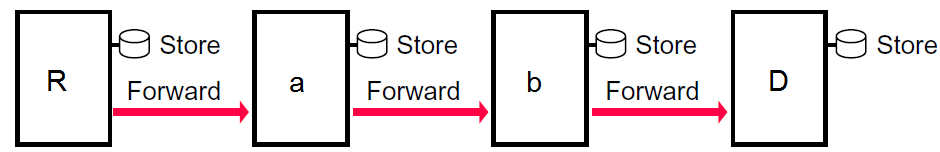
\includegraphics[width=0.9\textwidth]{figuras/cap_2/secao_1/armazena_envia.png}
\caption{Encaminhamento nas DTNs. Baseado em \cite{umrKehr}.}
\label{armazena_envia}
\end{figure}

A existência de dispositivos com hardware limitado torna importante o gerenciamento inteligente das mensagens acumuladas nos nós, pois, devido a limites de armazenamento, pode ser necessário excluir algumas em prol do armazenamento de outras. A mensagem que será apagada deve ser escolhida de forma a amenizar ocorrências de situações difíceis de prever, como apagar uma mensagem instantes antes de se encontrar com o destinatário.

Observa-se a importância dos contatos nas DTNs, pois a troca de mensagens só é possível na ocorrência dos mesmos. Como visto em \cite{rfc4838}, os contatos podem ser classificados de acordo com sua previsibilidade:

\begin{itemize}
    \item \textbf{Previsíveis:} Como o próprio nome indica, podem ser previstos de alguma forma. As redes espaciais são bons representantes para esta categoria devido ao fato de ser possível determinar, precisamente, o correto momento do envio e recepção de mensagens visto o comportamento cíclico dos astros;
    \item \textbf{Imprevisíveis:} São totalmente ou parcialmente estocásticos, ou seja, não é possível determinar, precisamente, quando e onde irão ocorrer. Redes onde os nós não possuem um padrão de comportamento bem definido representam esta categoria, sendo um exemplo as redes Ad Hoc.
\end{itemize}


Apesar de serem comumente encontradas na literatura como Redes Tolerantes a Atrasos e Desconexões, existem outras terminologias, tais como: Redes com Conectividade Eventual, Redes Desconectadas e Redes com Conectividade Transiente. Recentemente, o termo DTN também pode ser encontrado como Disruption-Tolerant Networking e é oriundo de atribuições realizadas pela DARPA, a Agência de Projetos de Pesquisa Avançada de Defesa dos Estados Unidos, que faz altos investimentos em pesquisas relacionadas às DTNs, principalmente para uso militar \cite{krishnan2007spindle, sehl2013viability}.

\newpage
\subsection{Arquitetura}

A definição de uma arquitetura básica capaz de atender e amenizar os problemas enfrentados nas DTNs é muito importante. Tal trabalho foi realizado por \cite{fall2003delay} e é alvo de inúmeros estudos e complementações. Em seu artigo, Fall propõe uma arquitetura baseada no armazenamento e reenvio de mensagens e utilização de \emph{gateways}, responsáveis por interconectar regiões\footnote{Regiões são definidas como áreas onde há uma maior homogeneidade entre as características dos nós.} de uma DTN.

Como visto em \cite{rfc5050} e \cite{umrKehr}, a troca de mensagens entre os nós é implementada, nas DTNs, por meio de um modelo em camadas baseado no modelo OSI, assim como a Internet. O principal diferencial entre o modelo das DTNs e o da Internet é a existência da \emph{Camada de Empacotamento} (do inglês "Bundle Layer"), ilustrada na Figura \ref{camadas_dtn}. Esta camada é responsável pelo armazenamento temporário de mensagens, gerenciamento do \emph{buffer} de armazenamento utilizado pelos nós e abstração da troca de mensagens pelas aplicações que rodam sobre DTNs.

\begin{figure}[htp!]
\centering
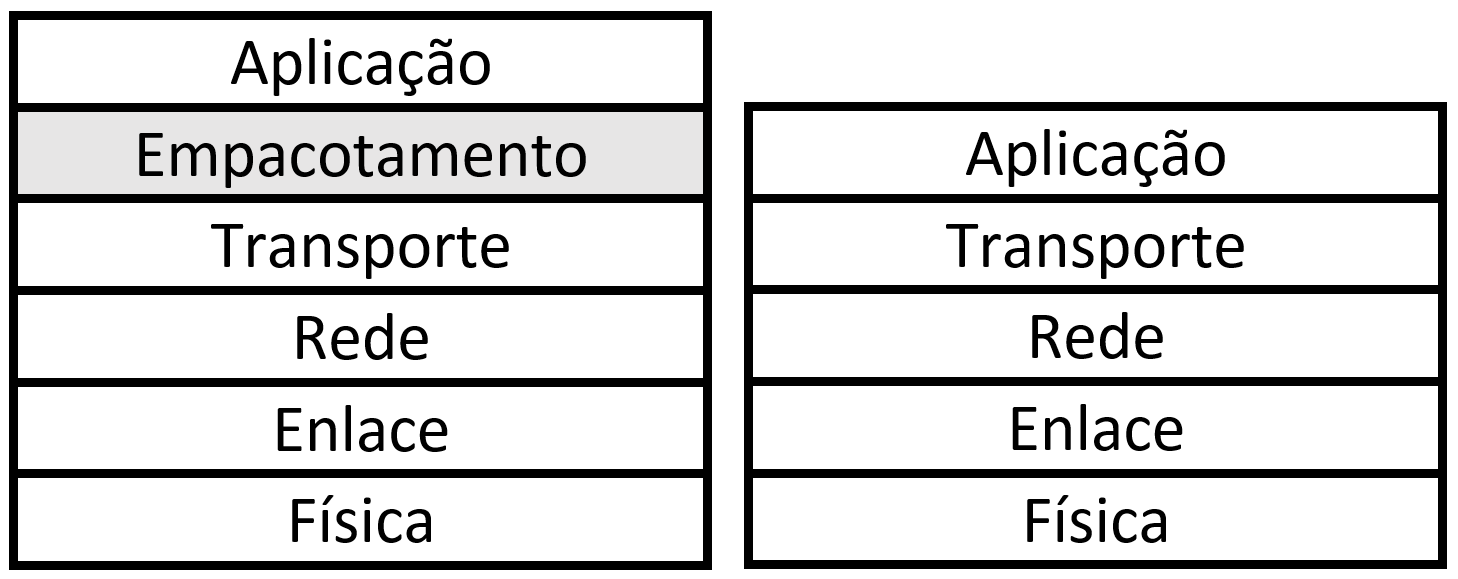
\includegraphics[width=0.7\textwidth]{figuras/cap_2/secao_1/camadas_dtn.PNG}
\caption{Pilha de camadas de comunicação das DTNs (esquerda) comparada com a da Internet (direita). Baseado em \cite{umrKehr}.}
\label{camadas_dtn}
\end{figure}

Os \emph{gateways} são dispositivos que compõem as DTNs capazes de armazenar e retransmitir mensagens utilizando diferentes protocolos de roteamento e transporte. Como exemplo, um \emph{gateway} pode receber uma mensagem de um nó utilizando os protocolos TCP e IP e retransmiti-la utilizando outros, como o SCTP e IP \cite{fall2003delay}. Seu uso se faz necessário pelo fato de DTNs de diferentes regiões executarem diferentes protocolos de comunicação, permitindo assim a interoperabilidade de protocolos existentes em arquiteturas distintas.

O modelo proposto por Fall prevê ainda o uso de tuplas para a identificação de objetos ou grupos deles. Elas possuem duas componentes. A primeira é responsável por identificar o nome de uma região e é estruturada de forma hierárquica e única. A segunda é responsável por identificar entidades ou grupo delas. Os \emph{gateways} ficam então responsáveis por armazenar tabelas de roteamento baseadas nessas tuplas, permitindo um mapeamento global, seja ele dinâmico ou estático, das regiões e otimização do redirecionamento das mensagens.

A Figura \ref{dtn_fall} ilustra a arquitetura proposta por Fall, onde existem quatro regiões (A, B, C e D) bem distintas, presença de diferentes dispositivos, identificados por tuplas, e meios de encaminhamento. O cenário apresentado é bastante diversificado, indo desde o transporte de mensagens por meio de um ônibus, identificado pela tupla \{B, R4\}, até a comunicação com um satélite artificial, identificado pela tupla \{D, Satellite\}.

\begin{figure}[htp!]
\centering
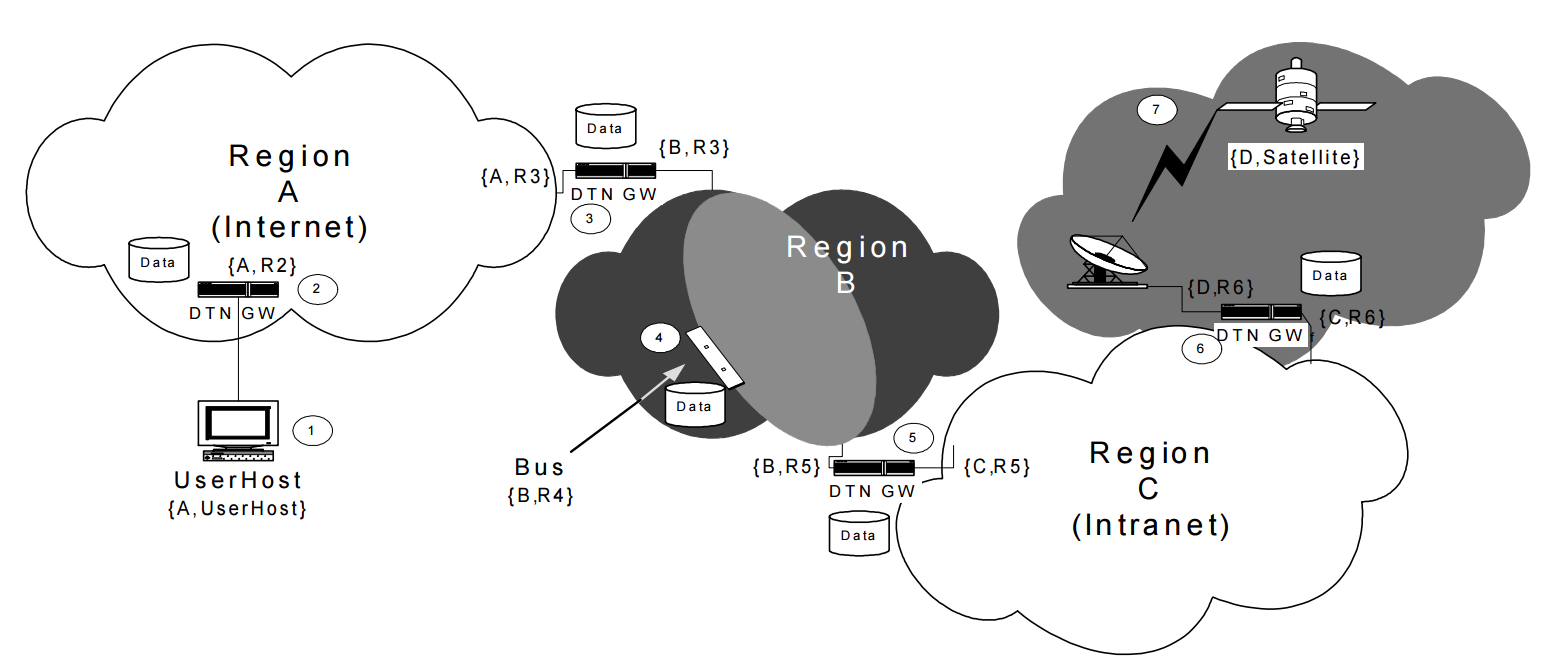
\includegraphics[width=1\textwidth]{figuras/cap_2/secao_1/dtn_fall.png}
\caption{Arquitetura de DTN utilizando gateways para interconectar DTNs com diferentes protocolos de comunicação \cite{fall2003delay}.}
\label{dtn_fall}
\end{figure}

O papel dos \emph{gateways} é reforçado na Figura \ref{dtn_fall}. Os \emph{gateways} identificados na região B como \{B, R3\} e \{B, R5\} armazenam temporariamente as mensagens enquanto o ônibus \{B, R4\} as transporta de um para o outro.

\subsection{Encaminhamento de Mensagens}
\label{subsec:encaminhamento_mensagens}
Protocolos de Encaminhamento de mensagens são importantes em qualquer arquitetura de redes de computadores. A partir deles as mensagens são comutadas nó a nó na rede até que elas sejam entregues aos seus destinos. Nas DTNs isso não é diferente e diversos protocolos de encaminhamento foram desenvolvidos voltados para as características dessas redes.

Os protocolos de encaminhamento destinados às DTNs podem ser divididos em dois grupos principais: Probabilísticos e Não-Probabilísticos. Cada grupo possui características próprias, como taxa de entregas de mensagens, taxa de utilização de buffers e controle da quantidade de cópias de mensagens existentes na rede.

\subsubsection{Protocolos Probabilísticos}

Protocolos Probabilísticos fazem uso de dados estatísticos calculados por meio de informações obtidas da própria rede, como taxa de encontro entre cada um dos nós, quantidade de retransmissões das mensagens, taxas de sucesso e insucesso das transmissões e quantidade de cópias existentes de uma determinada mensagem na rede. Esses protocolos utilizam critérios para determinar, a partir dos dados, os melhores critérios de encaminhamento a serem utilizados.

Por utilizarem dados estatísticos, os Protocolos Probabilísticos tendem a tomar melhores decisões de acordo com o reconhecimento da rede, pois a maior quantidade de dados obtida com o tempo melhora os dados estatísticos e, consequentemente, melhora as decisões.

Entre os Protocolos Probabilísticos, destaca-se o protocolo Prophet:

\begin{itemize}
    \item \textbf{Prophet:} De acordo com \cite{lindgren2003probabilistic}, este protocolo utiliza o histórico de encontros entre os dispositivos para a tomada de decisão de roteamento. Numa rede que utiliza este protocolo, cada um dos nós armazena uma lista com todos os nós que já foram encontrados e uma \emph{Previsibilidade de Entrega} que é calculada de acordo com a quantidade de encontros entre os nós e decai quando eles não entram em contato por um determinado tempo. Esse protocolo utiliza a propriedade da transitividade, pois se um determinado nó \emph{R} possui mensagens para um nó \emph{D} que ele nunca se encontrou, mas um nó intermediário \emph{I} se encontra constantemente com \emph{D}, para \emph{R} o nó \emph{I} terá maior relevância na propagação da mensagem do que um outro nó \emph{N} que nunca se encontrou com \emph{D};
    %\item \textbf{MaxProp \cite{burgess2006maxprop}:} Ainda sendo estudado.
\end{itemize}

\newpage

\subsubsection{Protocolos Não-Probabilísticos}

Protocolos Não-Probabilísticos caracterizam-se pela ausência do uso de dados estatísticos na retransmissão das mensagens, destacando-se os seguintes:

\begin{itemize}
    \item \textbf{Epidemic Routing:} Segundo \cite{vahdat2000epidemic}, este protoloco parte do pressuposto de que quanto mais cópias de uma mesma mensagem existirem na rede, maiores serão as chances de entrega. Numa rede que executa esse protocolo, os nós retransmitem todas as mensagens armazenadas em \emph{buffer} quando entram em contato com outro, inundando a rede com diversas cópias. Problemas como o congestionamento da rede e o estouro de \emph{buffers} são constantes, fazendo necessário o uso de técnicas para a redução desses problemas, como o uso de indicadores (\emph{beacons}) de entrega da mensagem, uso de políticas para priorizar umas em relação à outras (como o tempo de criação) e uso de um número máximo de saltos que uma mensagem pode sofrer;
    \item \textbf{Spray-and-wait:} Como visto em \cite{spyropoulos2005spray}, este protocolo foi desenvolvido com o intuito de reduzir a quantidade de duplicatas de uma mensagem na rede e as taxas de estouro de \emph{buffers} nos dispositivos. Basicamente, existem duas fases, uma de pulverização e outra de espera. Na fase de pulverização os nós vão disseminando a mensagem pela rede até que um número limitado de nós esteja armazenando a mensagem. Na fase de espera, os nós só retransmitem a mensagem quando o nó destino é encontrado. A mobilidade dos nós deve ser consideravelmente alta, pois nós pouco móveis podem acabar fazendo com que o destinatário nunca seja alcançado;
    \item \textbf{Direct Contact:} Em \cite{spyropoulos2007spray}, é visto que neste protocolo as mensagens só são retransmitidas se o remetente se encontra com o destinatário. Os problemas de congestionamento e estouro \emph{buffers} existente no protocolo epidêmico são praticamente resolvidos, mas as chances de entrega das mensagens são muito reduzidas, pois remetente e destinatário podem nunca se encontrar.
\end{itemize}

\subsubsection{Comparação entre os Protocolos Probabilísticos e Não-Probabilísticos}

Intuitivamente, percebe-se uma grande vantagem dos Protocolos Probabilísticos em relação aos Não-Probabilísticos.

Os Probabilísticos, com o uso de estatísticas provenientes da própria rede gerenciam de forma inteligente as retransmissões de mensagens, possuem baixas taxas de estouro de buffer, menor quantidade de duplicatas de mensagens e maiores taxas de entrega em relação aos Não-Probabilísticos. Sua característica adaptativa o torna mais eficiente de acordo com o tempo, mas, em redes recém implementadas, as probabilidades de erro e perdas de mensagens são elevadas.

Os protocolos Não-Probabilísticos baseiam-se primordialmente na mobilidade dos nós e em técnicas simples de roteamento de mensagens. Essas características os tornam problemáticos em redes com nós mais estáticos, mas de implementação simplificada em relação aos Probabilísticos. Mesmo aumentando as chances de entregas, a inundação da rede realizada pelo Protocolo Epidêmico pode acabar afogando os nós, fazendo com que o desempenho não seja satisfatório devido às altas taxas de estouro dos buffers.

\subsection{Aplicações Existentes}
\label{sec:aplicacoes}

Na literatura sobre DTNs inúmeros casos de aplicações são referenciados. Nesta subseção são apresentados alguns desses casos.

\subsubsection{O ZebraNet}

O projeto ZebraNet tem como objetivo monitorar a vida de zebras. Por meio de colares colocados nesses animais é feita a coleta e o armazenamento de dados referentes às suas vidas em seu habitat, permitindo uma análise detalhada do comportamento deles \cite{juang2002energy} \cite{zhang2004hardware}.

Assim como todo animal em seu ambiente natural, as zebras se movimentam de uma forma que a coleta de dados por humanos é dificultada, principalmente pelo fato de que os seres humanos afugentam esses animais. A solução para isso é obtida por meio do uso de colares que são colocados nas zebras e funcionam como nós de uma grande rede DTN. 

O encaminhamento das mensagens pelos dispositivos é feito de forma hierárquica. A posição dos nós dentro dessa hierarquia é baseada na quantidade de vezes que este se encontrou com a estação de coleta de dados. Quanto maior essa quantidade de encontros com a base, mais próximo do topo o nó estará da hierarquia. Estar próximo do topo significa que o nó tende a se encontrar muito com a base e, consequentemente, possui grande chance de se encontrar novamente num futuro próximo. A partir daí, quando um nó se encontra com dois dispositivos, um próximo do topo e outro distante, será dada a preferência de encaminhamento para o nó mais próximo do topo, visto que maiores são as chances dele se encontrar com a base num futuro próximo \cite{juang2002energy}.

A Figura \ref{zebra} apresenta uma zebra com o colar desenvolvido pelo projeto. Pode ser visto que ele foi desenvolvido para se adequar ao pescoço desses animais. Além disso, instalar esses dispositivos nesses animais exige que ele seja o mais confortável possível, visto que qualquer irritação gerada pelo mesmo pode influenciar nos resultados obtidos pelo projeto.

\begin{figure}[htp!]
    \centering
    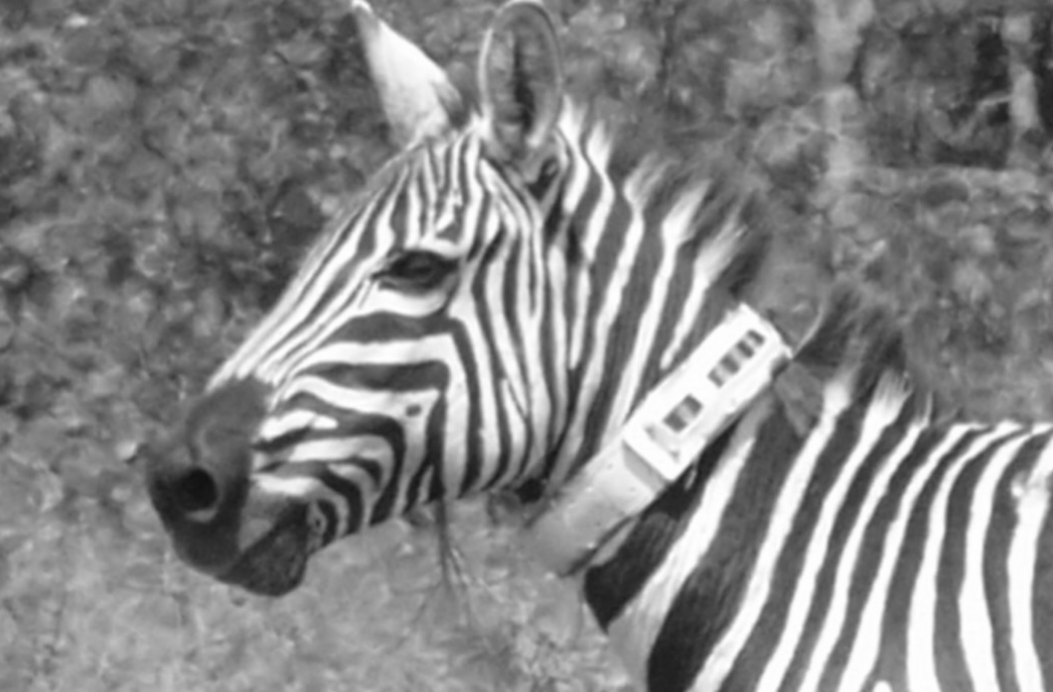
\includegraphics[width=0.8\textwidth]{figuras/cap_2/secao_1/zebranet.png}
    \caption{Zebra com o colar desenvolvido pelo projeto ZebraNet \cite{zhang2004hardware}.}
    \label{zebra}
\end{figure}

O estudo da vida das zebras por meio do ZebraNet trás contribuições para diversas áreas de estudo, como ecologia, biologia e redes de computadores.

\subsubsection{Redes Móveis Ad Hoc}

Um caso de aplicação das DTNs são as Redes Móveis Ad Hoc (do inglês "Mobile Ad Hoc Netwrok" ou MANET). Em geral, uma MANET, é uma infraestrutura autônoma composta por dispositivos móveis sem fio que trocam dados sem a necessidade de um elemento intermediador, como nas redes WiFi em modo Ad Hoc.

\subsubsection{O Wizzy Digital Courier}

Prover conectividade em áreas muito distantes de qualquer infraestrutura de Internet é um grande desafio e, já não é de hoje, que conectar regiões emergentes, como áreas rurais, atraem a atenção de pesquisadores \cite{tierProject}.

O Wizzy Digital Courier, nada mais é do que um projeto responsável por prover conectividade com a Internet por meio de uma DTN a escolas localizadas em locais remotos na África do Sul. Para isso, o projeto faz uso de uma motocicleta, equipada com dispositivos de armazenamento móveis, que realiza o encaminhamento dos dados até a cidade mais próxima que possui conexão com a Internet de alta capacidade. Geralmente, o processo de encaminhamento das mensagens com a motocicleta leva muitas horas, todavia é uma forma barata e acessível para os padrões econômicos da região. \cite{jain2004routing}


\subsubsection{Comunicação Espacial}

A comunicação entre satélites em órbita, estações, naves espaciais, sondas interplanetárias e telescópios depende da movimentação destes elementos e dos próprios movimentos dos corpos celestes, como planetas e estrelas. Os movimentos de rotação e translação dos planetas, estrelas e satélites naturais podem, eventualmente, gerar períodos de conexão e desconexão com centros localizados na Terra. A mobilidade e frequentes desconexões são características são típicas das DTNs e são marcantes neste cenário.

A Figura \ref{satelites} mostra um exemplo de sistema de comunicação interplanetária composto por dois satélites artificiais. Em um determinado instante \emph{a} do tempo, os satélites conseguem trocar dados pois não existem barreiras físicas suficientemente fortes para inviabilizar a comunicação. No instante \emph{b} a comunicação é inviabilizada pois o planeta marciano encontra-se entre os dois dispositivos.

\begin{figure}[htp!]
    \centering
    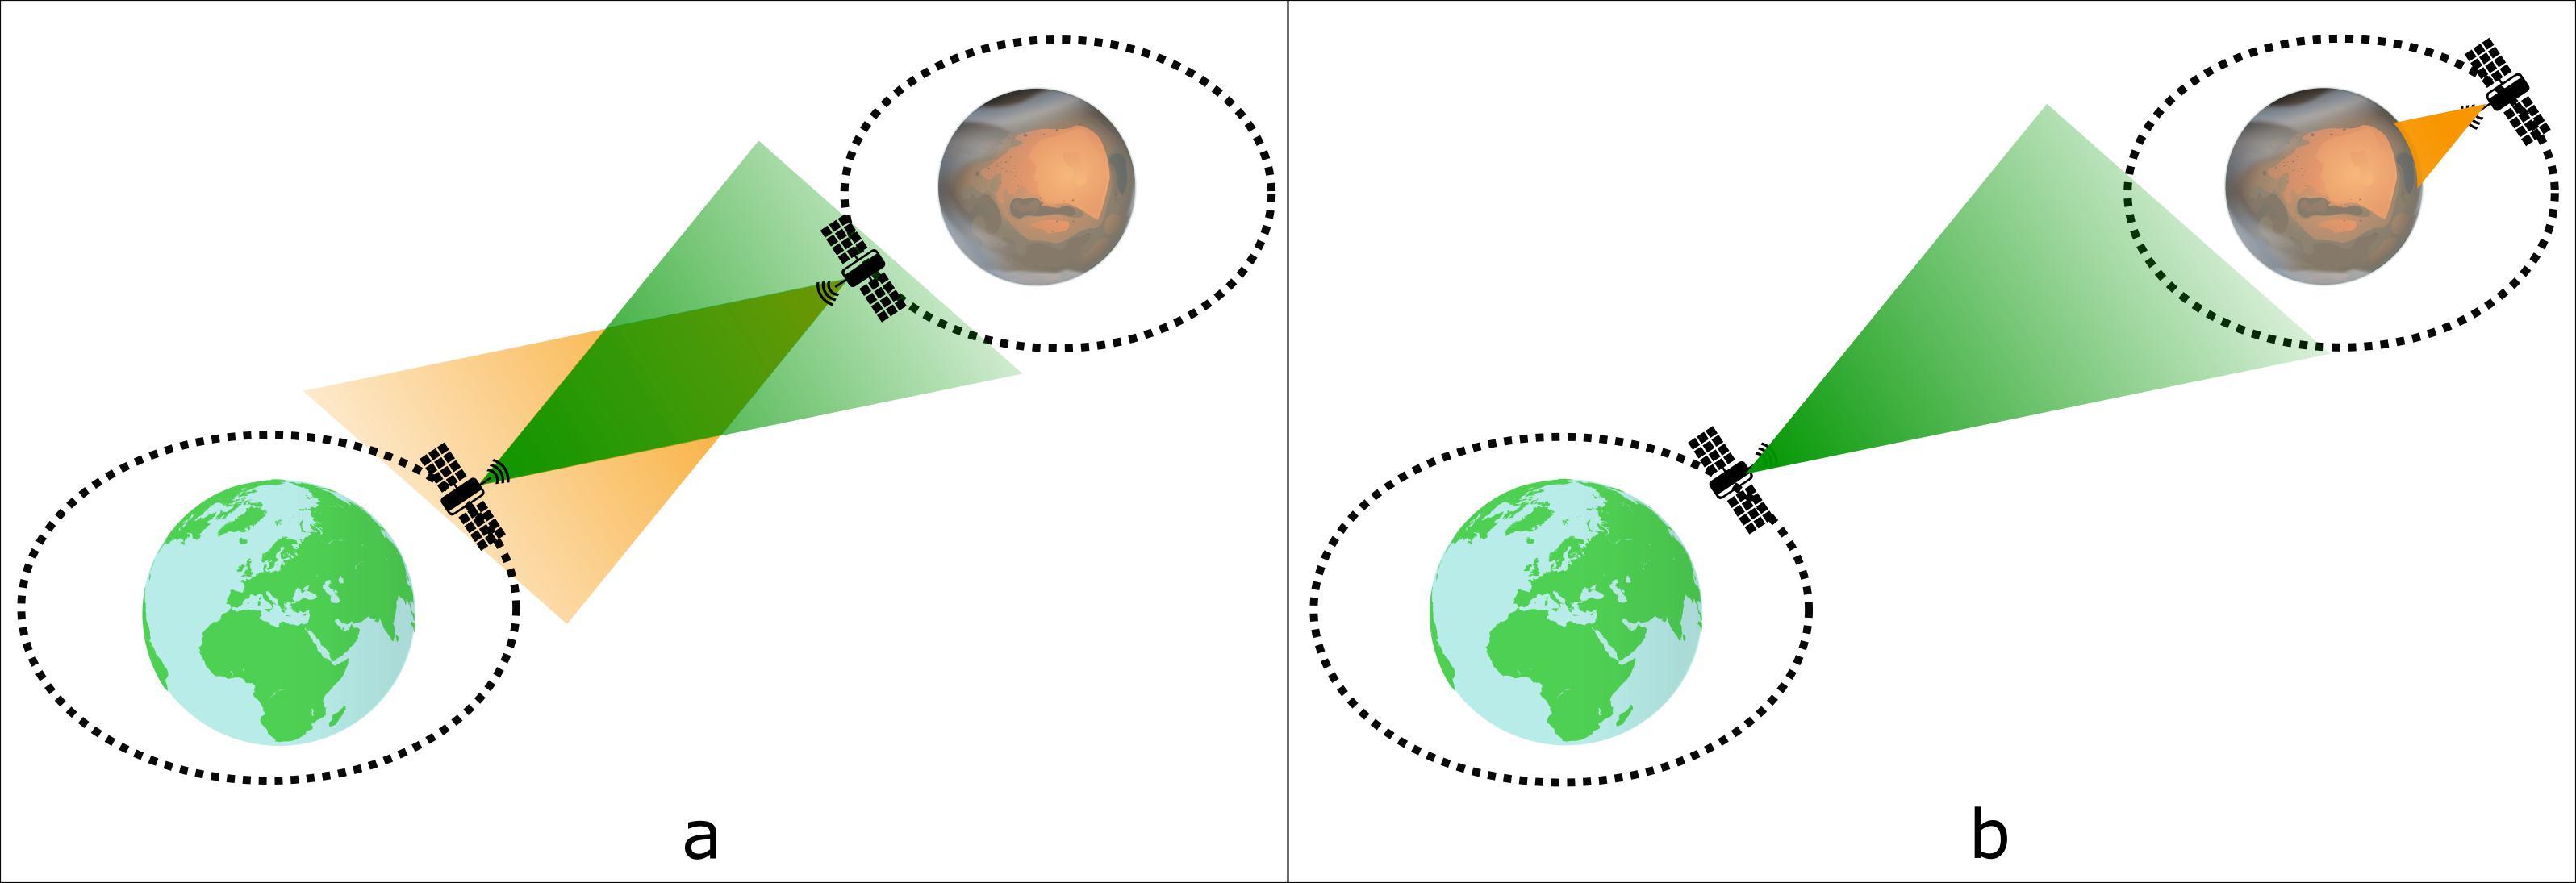
\includegraphics[width=1\textwidth]{figuras/cap_2/secao_1/satelites.png}
    \caption{Exemplo de comunicação espacial.}
    \label{satelites}
\end{figure}

\subsection{Principais Desafios}

As DTNs são conhecidas ainda como CHANTS ("Challenged NeTworks", ou "Redes com Desafios", em português) \cite{chen2006hybrid}. Tal atribuição remete, principalmente, a grande quantidade de desafios envolvidos na gerência e implementação de protocolos de roteamento para esse tipo de rede.

A característica móvel dos dispositivos torna necessário o uso de baterias que possuem capacidade de armazenamento de carga limitada. Essa limitação é um desafio inerente das DTNs e depende do uso de mecanismos de recarga e desenvolvimento de técnicas visando o consumo inteligente da energia por parte dos dispositivos.

O gerenciamento inteligente do consumo das baterias é, atualmente, alvo de grandes pesquisas, como pode ser visto em \cite{denis_artigo}. Silva, em seu artigo, realiza uma análise do consumo dos principais protocolos de roteamento das DTNs e, como principal resultado, afirma que a busca por dispositivos é grande responsável pelo consumo das baterias e aponta um intervalo ótimo de 32 segundos entre as buscas.

Em \cite{denis_artigo} não são considerados fatores como a probabilidade de contatos em regiões geográficas. A busca por dispositivos em áreas de maior quantidade de contatos registrada possui maior probabilidade de sucesso do que em áreas com menor quantidade, logo é de importante valia o estudo da dinamização do intervalo de busca proposto por Silva. Para tanto, podem ser utilizadas teorias relacionadas ao \emph{Referenciamento Geográfico} e \emph{Gradiente de Concentração} para o mapeamento da quantidade de contatos das regiões geográficas. Essas teorias são explanadas nas seções subsequentes.


\newpage
\section{Gradientes de Concentração}
\label{sec:gradientes_de_concentracao}

Nesta seção o conceito de Gradientes de Concentração é explanado por meio da contextualização e definição aceca deste tema. Após isso, é apresentada uma proposta de aplicação deste conceito na área de \emph{Redes Tolerantes a Atrasos e Desconexões}.

\subsection{Contexto}

Existem particularidades nas propriedades físico-químicas quando se trabalha com compostos. Intuitivamente, exemplifica-se que, ao se fazer uma bebida - um simples suco natural - é preciso realizar a mistura de determinados ingredientes, como água, açúcar e a polpa da fruta característica pelo tipo de suco.

O processo de mistura é, na maioria das vezes, tão simples que os indivíduos nem percebem ou não levam em consideração a complexidade envolvida. Isso se deve ao fato de ser simples do ponto de vista macroscópico. Partindo de um minúsculo ponto de vista, o molecular, as moléculas de água, portadoras de propriedades particulares, são capazes de interagir com os cristais de açúcar, dissolvendo-os até um ponto de equilíbrio, que se dá quando não é mais possível continuar esse processo, ou seja, não existem mais cristais, mas sim moléculas de sacarose\footnote{Substância extraída da cana-de-açúcar e beterraba, comum em produtos alimentícios, como adoçante de alimentos e bebidas, geleias, doces e, até mesmo, xaropes.} espalhadas pela água utilizada. 

A mistura de açúcar com água possui, inicialmente, uma heterogeneidade, existindo assim um \emph{Gradiente de Concentração}, ou seja, uma diferença de concentração (os cristais de açúcar possuem maiores concentrações de moléculas de sacarose do que a água pura) entre os elementos envolvidos, dando partida ao processo de dissolução dos cristais. Esse processo ocorre até um ponto que a mistura de água e açúcar se torne uniforme, ou homogênea, de forma que não exista mais um \emph{Gradiente de Concentração}.

\subsection{Definição}

Em química, o \emph{Gradiente de Concentração} indica a alteração no valor da concentração de determinada substância por unidade de espaço. Este conceito pode ser utilizado em diversas áreas, como física, biologia e geografia. Tal gradiente é, geralmente, representado de forma gráfica \cite{concentrationGradient}.

A mistura de água com açúcar caracteriza-se por uma situação semelhante a representada na Figura \ref{agua_acucar_copo} (onde as bolinhas vermelhas representam as moléculas de sacarose e, o fluido em azul, a água).

\begin{figure}[htp!]
\centering
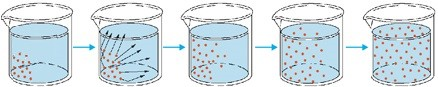
\includegraphics[width=0.80\textwidth]{figuras/cap_2/secao_2/agua_acucar_copo.jpg}
\caption{Difusão de moléculas de sacarose num copo de água \cite{concentrationGradient}.}
\label{agua_acucar_copo}
\end{figure}

É atribuído o nome \emph{difusão} ao processo representado na Figura \ref{agua_acucar_copo} \cite{concentrationGradient}. Não é objetivo deste trabalho explanar sobre as razões desse fenômeno. Em suma esse é um comportamento estocástico, natural e acontece a todo momento na natureza e no corpo humano.

Baseando-se em \cite{concentrationGradient}, é possível discretizar o processo de difusão da sacarose, obtendo o resultado visto na Figura \ref{modeculas_sacarose_agua}, onde a água pode ser vista na cor branca e as moléculas de sacarose na cor azul. É observada uma mistura gradativa do quadro esquerdo para o direita até que uma mistura quase perfeita seja alcançada.

A Figura \ref{gradiente_modeculas_sacarose_agua} apresenta os \emph{Gradientes de Concentração} para cada uma das etapas apresentadas na Figura \ref{modeculas_sacarose_agua}, baseado-se no material de \cite{concentrationGradient}. Nota-se, no gradiente à esquerda, uma grande concentração de substância na parte de baixo. A grande concentração ainda existe no gradiente do meio, mas a substância começou a se difundir para a parte superior. No último, a direita, há apenas uma cor uniforme, pois o gradiente já não existe mais, ou seja, as moléculas já se difundiram completamente.

\begin{figure}[htp!]
\centering
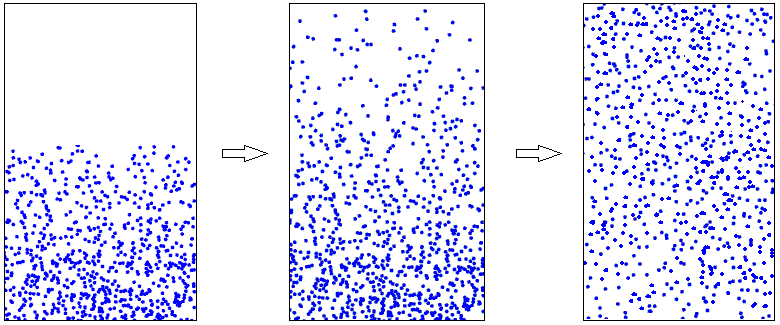
\includegraphics[width=1.0\textwidth]{figuras/cap_2/secao_2/modeculas_sacarose_agua.png}
\caption{Difusão de moléculas de sacarose num copo de água.}
\label{modeculas_sacarose_agua}
\end{figure}

\begin{figure}[htp!]
\centering
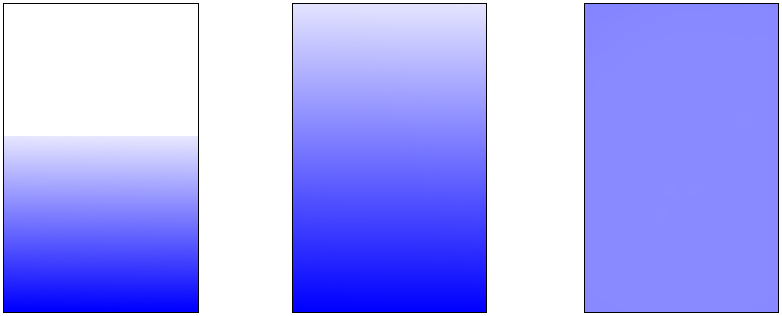
\includegraphics[width=1.0\textwidth]{figuras/cap_2/secao_2/gradiente_modeculas_sacarose_agua.png}
\caption{Gradientes de Concentração da difusão de moléculas de sacarose. A cor branca indica ausência de moléculas e, a cor azul intensa, alta concentração.}
\label{gradiente_modeculas_sacarose_agua}
\end{figure}
\newpage
\subsection{Aplicabilidade nas DTNs}

Na área de interesse deste trabalho, um \emph{Gradiente de Concentração} pode ser utilizado para representar dispositivos por unidade de área, permitindo representar regiões com muitos dispositivos como tendo maior concentração em relação a outras com menos dispositivos.

Os gradientes apresentados na Figura \ref{gradiente_modeculas_sacarose_agua} possuem uma única dimensão. Para o contexto geográfico, essa representação discretizada não traz resultados satisfatórios e, muito menos, intuitivos, principalmente pelo fato de que o mapeamento geográfico se basear em duas ou, até mesmo, três dimensões.

A Figura \ref{mapa_dispositivos} mostra um mapa com vários dispositivos distribuídos, representados por pontos verdes nomeados. Existe, no mapa, uma distribuição não uniforme de dispositivos, que é ainda mais evidenciada com a divisão em regiões de igual tamanho apresentada na Figura \ref{mapa_regioes_dispositivos}.

A concentração de dispositivos pode ser dada pela quantidade de nós de uma área dividida pela quantidade total de dispositivos da rede. A partir daí, é possível construir a Figura \ref{gradiente_mapa_regioes_dispositivos}, que representa um \emph{Gradiente de Concentração} bidimensional para o mapa inicialmente apresentado na Figura \ref{mapa_dispositivos}. A representação proporciona, de forma intuitiva, uma visualização discretizada de áreas com maior e menor incidência de dispositivos.

\begin{figure}[htp!]
\centering
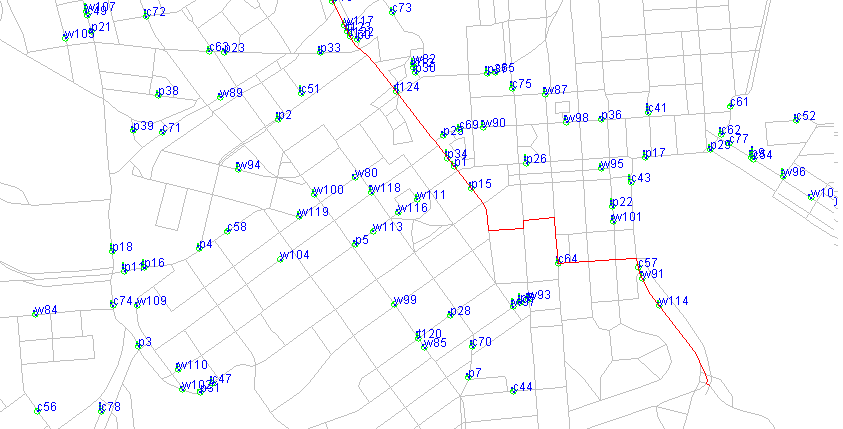
\includegraphics[width=1.0\textwidth]{figuras/cap_2/secao_2/mapa_dispositivos.png}
\caption{Mapa fictício com diversos dispositivos distribuídos por ele.}
\label{mapa_dispositivos}
\end{figure}

\begin{figure}[htp!]
\centering
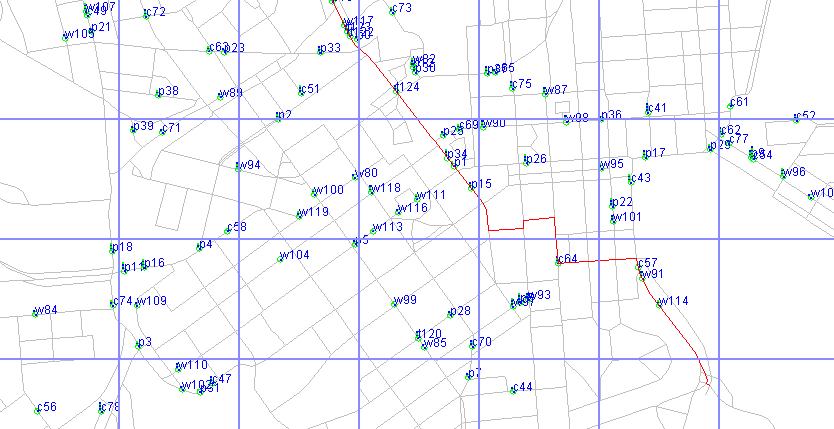
\includegraphics[width=1.0\textwidth]{figuras/cap_2/secao_2/mapa_regioes_dispositivos.png}
\caption{Mapa da Figura \ref{mapa_dispositivos} dividido em regiões de igual tamanho.}
\label{mapa_regioes_dispositivos}
\end{figure}

\begin{figure}[htp!]
\centering

\includegraphics[width=1.0\textwidth]{figuras/cap_2/secao_2/gradiente_mapa_regioes_dispositivos.png}
\caption{Gradiente de Concentração baseado na Figura \ref{mapa_regioes_dispositivos}. A cor branca indica ausência de dispositivos e, a cor azul intensa, alta concentração.}
\label{gradiente_mapa_regioes_dispositivos}
\end{figure}

Cada região pode ser identificada e sua respectiva concentração definida por um número, inteiro ou real, responsável por indicar a intensidade desta, similar a cor. Quanto maior a concentração, maior este número e ainda maiores são as chances de encontrar algum dispositivo ao realizar uma busca. Portanto, pode-se reduzir ou aumentar a intensidade de buscas em determinadas áreas de acordo com a concentração, proporcionando um ajuste adaptativo de um importante fator no consumo de energia dos dispositivos: o intervalo de busca por dispositivos.

\subsection{Desafio}
\label{subsec:gradientes_desafios}
A representação da rede por meio de um gradiente tem como principal desafio a montagem do mesmo. O uso de técnicas de geolocalização são necessárias para o referenciamento e definição de regiões geográficas. Tais técnicas são detalhadas na Seção \ref{sec:GNSS}.

A construção do gradiente pode ser feita de forma independente entre os dispositivos que, ao entrarem em contato, trocam informações de seus gradientes numa forma semelhante a uma prosa: “Olha, eu sei que já ocorreram mais contatos na região X do que na Y, talvez isso possa ser útil para você.” e o outro responde “Legal. Como agradecimento, dar-lhe-ei as informações das regiões que já passei.”. 

Ao final de muitos contatos, os dispositivos terão um grande mapa das regiões onde eles já passaram tendo informações de localidades com maior e menor incidência de contatos, permitindo o ajuste dinâmico de fatores que influenciam no consumo de energia.

\section{Sistemas de Navegação por Satélites}
\label{sec:GNSS}
Nesta seção é apresentado o referencial teórico sobre Sistemas de Navegação por Satélites, seus princípios básicos, funcionamento e como podem ser aplicados no desenvolvimento da técnica adaptativa objetivada neste trabalho.

\subsection{Contexto e Definições}

A última década foi marcada pela popularização e evolução dos dispositivos móveis, principalmente os \emph{smartphones}. Esses dispositivos contam com diversas funcionalidades de software e hardware úteis para o dia a dia dos usuários, incluindo, em sua gigantesca maioria, serviços de geolocalização, que, por sua vez, dão ao usuário informações sobre a sua localização geográfica corrente.

Para o ser humano moderno, a possibilidade de saber qual a sua posição atual no mundo traz inúmeras vantagens que vão muito além de saber se está próximo de um estabelecimento que o mesmo está procurando para realizar as compras do mês. O acesso a essa informação traz a humanidade um leque de possibilidades, que são ainda mais ampliadas com o uso de uma rede de computadores. Como exemplo, podemos ter acesso à informações sobre o clima local, saber sobre os estabelecimentos próximos, calcular rotas precisas a partir da posição do usuário, associar o local a fotos e vídeos, e muito mais. Além disso, sistemas de georreferenciamento fazem o uso de imagens de satélites para determinar os limites de bairros e casas visando gerar informações de limites e posicionamento.

Existem, atualmente, dois principais Sistemas de Navegação por Satélites (do inglês "Global Navigation Satellite Systems" ou GNSS) funcionais responsáveis por permitir a descoberta de informações sobre o posicionamento de objetos no globo: O NAVSTAR-GPS (do inglês "Navigation Satellite with Time And Ranging Global Positioning System"), comumente conhecido apenas como GPS, e o GLONASS (sigla de origem russa para "Sistema de Navegação Global por Satélite"). 

%Ambos os sistemas necessitam do uso de receptores específicos, tornando obrigatório a existência de um hardware especial para cada um. \cite{vaz2013comparaccao}

\subsection{Referenciando a Posição de um Objeto no Globo}

Qualquer ponto na Terra pode ser referenciado por meio de um Sistema de Coordenadas Geográficas. De todos os modelos existentes o mais comum e prático é o baseado em linhas imaginárias conhecidas como \emph{meridianos} e \emph{paralelos}. Os meridianos cortam o globo do polo geográfico norte ao polo geográfico sul, já os paralelos são linhas ortogonais\footnote{Linhas que formam um ângulo de 90º ao se cruzarem.} aos meridianos. De todos os paralelos e meridianos que podem ser traçados na terra, destacam-se o Meridiano de Greenwich, que divide a terra em um lado ocidental e outro oriental, e o Paralelo da Linha do Equador, que divide a terra em polo sul e polo norte. \cite{fitz2008geoprocessamento}

\begin{figure}[htp!]
\centering
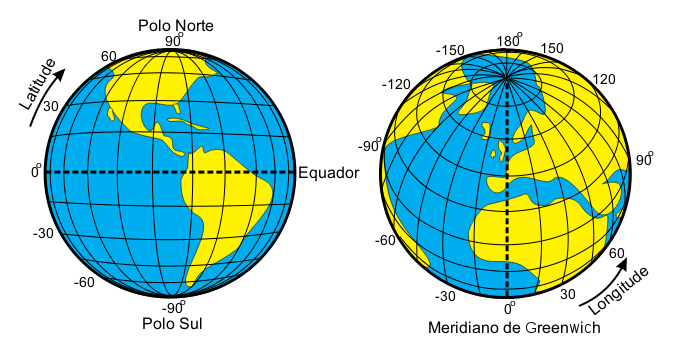
\includegraphics[width=0.80\textwidth]{figuras/cap_2/secao_3/latitude_longitude.png}
\caption{Latitude e Longitude}
\label{latitudeLingitude}
\end{figure}

A distância de qualquer ponto até a Linha do Equador é chamada de latitude e é medida em graus e varia de 0 a 90 graus, tanto para o norte (N) quanto para o sul (S). Para determinar a latitude de um ponto no globo, é preciso calcular o ângulo formado entre a linha do equador e uma reta que passa pelo ponto desejado e pelo centro da terra. Caso o ponto esteja em cima da linha do equador, não teremos a formação de um ângulo e, portanto, ele está na latitude 0º. \cite{fitz2008geoprocessamento}

Infelizmente, apenas com a latitude, não é possível determinar a posição exata de um ponto no globo. Para resolver isso é utilizada uma outra medida, a longitude. Esta medida, por sua vez, representa a distância do ponto desejado até o Meridiano de Greenwich e é calculada de forma similar a realizada para latitude, mas varia de 0 a 180 graus para leste (E) e para oeste (W). Um ponto que se localiza em cima do Meridiano de Greenwich está na longitude de 0º. \cite{fitz2008geoprocessamento}

A Figura \ref{washingtonDC} apresenta a latitude e a longitude aproximada de Washington D.C., a capital dos Estados Unidos da América.

\begin{figure}[htp!]
\centering
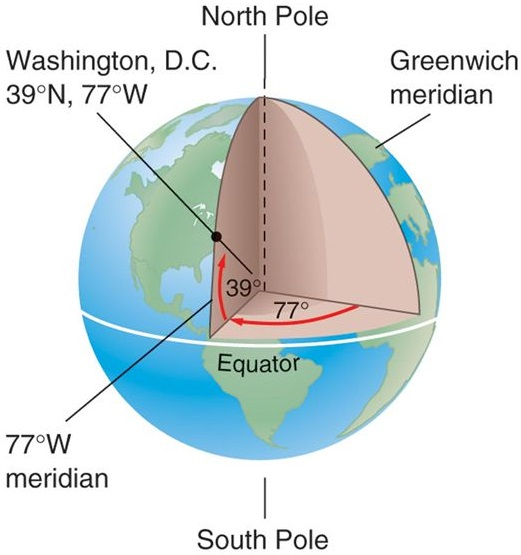
\includegraphics[width=0.60\textwidth]{figuras/cap_2/secao_3/washingtonDC.jpg}
\caption{Latitude e Longitude de Washington D.C.}
\label{washingtonDC}
\end{figure}

A distância em quilômetros de um grau a outro, que na latitude equivale a 111,12km e na longitude varia de 0 a 111,12km, torna necessário o uso de valores com várias casas decimais para representar com exatidão a posição de um objeto no globo. Para efeitos de simplificação, existe um modelo onde cada grau é dividido em duas componentes, uma de minutos (') e outra de segundos ("). Cada grau possui 60 minutos e cada minuto possui 60 segundos \cite{fitz2008geoprocessamento}. 

A divisão da latitude e da longitude em componentes torna possível simplificar a fala de uma coordenada geográfica. Como exemplo, a posição geográfica da \emph{Universidade Vila Velha} se dá na latitude 20.354043ºS e na longitude 40.299163ºW, que, quando convertido para o modelo utilizando minutos e segundos, se torna \newline 20º21'14,6"S e 40º17'57"W, respectivamente. A pronúncia do sistema em minutos e segundos é mais fácil de ser entendida e associada, pois discretiza os valores decimais muito longos que seriam necessários para referenciar um ponto no globo.

\subsection{O NAVSTAR-GPS}

O NAVSTAR-GPS, ou apenas GPS, como já foi introduzido, é uma tecnologia utilizada para determinar a posição geográfica de dispositivos no globo terrestre, fazendo uso de satélites artificiais, que funcionam como pontos de referência no espaço de posição muito bem conhecida. Além disso, foi desenvolvido pelo Departamento de Defesa dos Estados Unidos, o DOS (do inglês "Department of Defense"), está operacional desde 1994 e, devido ao tempo de operação, é mais popular em relação ao GLONASS.

A concepção do GPS permite que qualquer usuário situado na superfície terrestre, ou próximo dela, tenha a sua disposição, pelo menos, quatro satélites artificiais para serem rastreados, permitindo o conhecimento em tempo real da sua posição e uso sob condições climáticas extremas \cite{miguens1996navegaccao}. O GPS é um sistema passivo, pois não necessita que o usuário envie informações para os satélites, ficando estes responsáveis pelo envio dos sinais necessários.

Para calcular a posição de um usuário com precisão é utilizado um sistema de triangulação que faz uso da posição de três satélites e as suas respectivas distâncias até um receptor em terra. A distância do receptor até o satélite pode ser obtida por meio da medição do intervalo de tempo decorrido entre a transmissão dos sinais pelos satélites e a recepção pelo dispositivo receptor, sendo ela utilizada como raio de uma esfera cujo centro é a posição do satélite. A posição do usuário é o ponto em comum de interseção das três esferas, como ilustrado na Figura \ref{triangulacao_gps}.

\begin{figure}[htp!]
\centering
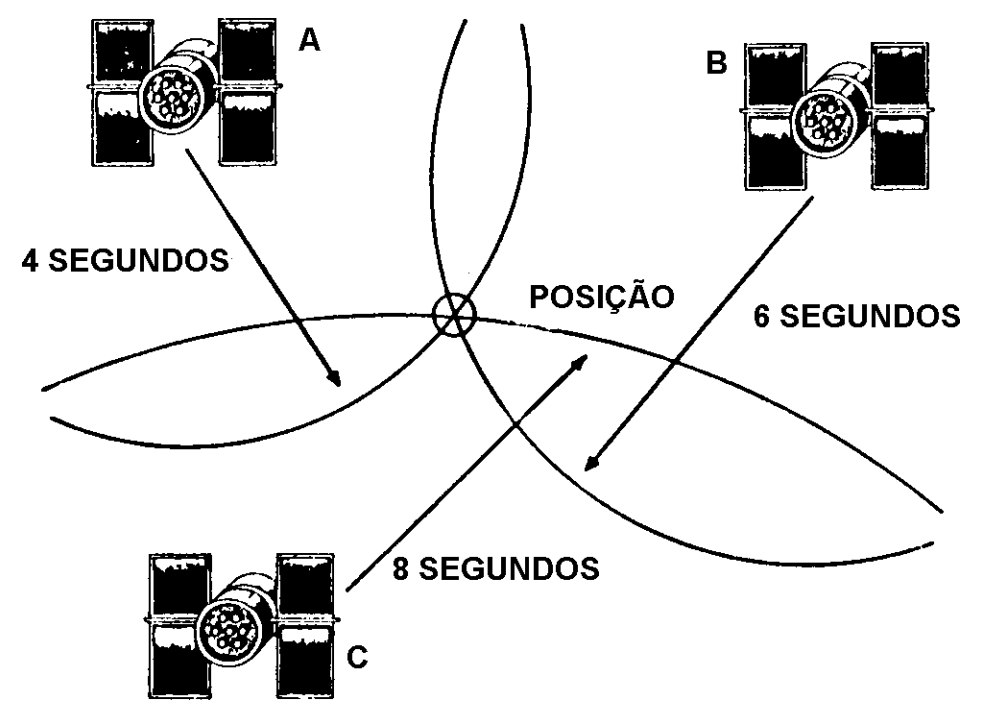
\includegraphics[width=0.60\textwidth]{figuras/cap_2/secao_3/triangulacao_gps.png}
\caption{Sistema de triangulação utilizado pelo NAVSTAR-GPS \cite{miguens1996navegaccao}.}
\label{triangulacao_gps}
\end{figure}

O cálculo do tempo decorrido entre a emissão do sinal e a recepção no dispositivo utilizado não é tão simples, pois exige a perfeita sincronização do relógio de todos os elementos envolvidos. Em situações práticas isso é muito improvável de acontecer e faz necessário o uso de mais um satélite para o processo, daí vê-se a importância da disponibilidade de, pelo menos, quatro satélites.

Não é objetivo deste trabalho realizar explanações muito específicas sobre o funcionamento do GPS. Detalhes de hardware, software e conceitos mais específicos podem ser encontrados em \cite{longley2009sistemas}.

\subsection{O GLONASS}

O GLONASS é uma tecnologia georreferenciamento de origem russa e, assim como o GPS, foi desenvolvido inicialmente para uso militar. Esse sistema só pôde ser considerado operacional em nível mundial no final 2011 e, a partir daí, começou lentamente a ser acoplado aos smartphones \cite{vaz2013comparaccao}, principalmente após o governo russo ter criado barreiras de importação para dispositivos que suportem apenas a tecnologia norte americana \cite{impostoRussia}.

O funcionamento da tecnologia russa é semelhante ao do GPS visto na Figura \ref{triangulacao_gps} e tem se tornado cada vez mais popular no mercado de dispositivos móveis e possui uma precisão muito próxima ao GPS \cite{vaz2013comparaccao}.

Até o ano de 2011, GPS e GLONASS eram totalmente incompatíveis entre-si, pois utilizavam técnicas de modulação e frequências diferentes. Entretanto, foi nesse ano que o GLONASS-K foi lançado e, por sua vez, possibilitou que dispositivos operem com as duas tecnologias utilizando um único receptor, visto que ele trabalha com frequências e modulações semelhante aos da tecnologia americana\newline \cite{kovar2011interoperable}.

\subsection{Contribuição para as Redes Tolerantes a Atrasos}

A descoberta da posição geográfica de dispositivos contribui de forma significativa em diversas áreas de pesquisa, entre elas as Redes Tolerantes a Atrasos. Conhecer a posição de cada um dos dispositivos que compõem uma DTN permite o levantamento de estatísticas de contatos ocorridos entre dispositivos em regiões preestabelecidas, abrindo mão para o gerenciamento inteligente de parâmetros que influenciam no consumo de energia dos dispositivos envolvidos.

A concentração pode ser calculada por meio da relação entre a quantidade total de contatos registrados e a quantidade de contatos ocorridos na região onde um nó se encontra. Quanto maior a concentração, maiores as chances de um dispositivo encontrar outro ao realizar uma busca e, portanto, é mais inteligente aumentar o consumo visando usufruir das oportunidades previstas. Quanto menor a concentração, menores as chances de encontrar outro dispositivo e, consequentemente, é mais inteligente economizar energia para momentos oportunos.

É importante ressaltar que o conceito de regiões apresentado na Seção \ref{sec:DTN} é diferente do que é utilizado para regiões geográficas. O primeiro refere-se a características relacionadas a protocolos, por exemplo, e aqui refere-se áreas geográficas.

\subsection{Consumo de Energia em Dispositivos Móveis}
\label{subsec:consumo_gps}
Visando o aumento da quantidade de mensagens entregues, é inerente no âmbito das DTNs tornar inteligente o consumo energético dos dispositivos. Isso implica numa análise do uso das baterias pelos dispositivos de GNSS quando considerada a contribuição proposta na Subseção anterior.

Em \cite{carroll2010analysis} foi realizado um estudo do consumo energético de diversos componentes existentes em smartphones, tais como CPU, memória RAM, memórias de armazenamento, além, é claro, de dispositivos de GPS, utilizando para isso técnicas e equipamentos de medição adequados.

Relativo ao consumo de dispositivos GPS, Carroll indica que, quando habilitados, eles consomem 143,1mW utilizando uma antena interna e 166,1mW quando utiliza-se uma antena externa. Ainda é explicitado no trabalho de Carroll que, quando desabilitados, os dispositivos GPS não realizam qualquer consumo de energia.

Outro resultado relevante apontado por Carroll é o de que não existem diferenças de consumo quando a quantidade de satélites visíveis é analisada. Sendo assim, é possível concluir que seus resultados podem ser utilizados em simulações sem a necessidade de simular a movimentação de satélites para aumentar o grau de realismo.

É visto que o estudo de Carroll é de importante valia na simulação da técnica desenvolvida neste trabalho, visto que ela baseia-se no uso de dispositivos de Georreferenciamento. Além disso, o trabalho referenciado permite aumentar o grau de realismo das simulações realizadas no que diz respeito ao consumo de energia. 

Para efeitos de simplificação, as simulações realizadas no capítulo \ref{cap:testes} consideram a média dos consumos apontados por Carrol, ou seja, 154,6mW.

\section{Conclusão do Capítulo}\label{sec:conclusao_cap_2}

A primeira seção deste capítulo apresentou um breve estudo sobre as DTNs, incluindo conceitos relacionados, arquitetura, aplicações e uma análise sobre o problema de energia existente. Além disso, ainda sobre as DTNs, os principais protocolos de disseminação foram descritos de forma sucinta.

Conceitos relacionados aos Gradientes de Concentração foram apresentados na seção subsequente a das DTNs. A explanação intuitiva foi utilizada visando facilitar o entendimento da analogia utilizada para a aplicação no ambiente das redes objetivadas neste trabalho.

Foi visto que o estudo e dinamização do intervalo de busca proposto por \newline \cite{denis_artigo} pode ser realizado a partir da análise da incidência de contatos em regiões previamente estabelecidas. Para tanto, foram apresentados conceitos sobre referenciamento geográfico, descrevendo sucintamente como referenciar posições no globo e as principais tecnologias de referenciamento existentes atualmente.

A importância da análise incremental apresentada neste capítulo se dá pelo principal problema existente nas DTNs: o consumo de energia. Não existem, atualmente, formas de solucioná-lo definitivamente, mas é possível desenvolver técnicas de software que visam realiza o consumo inteligente das baterias, que é o principal objetivo do presente trabalho.